\chapter{Enity Embeddigns}\label{chap:entity}

In this chapter, we try to explore different ways to train word embeddings for entities and terms jointly. We use the word embedding and graph embedding models explained in the previous chapter, on annotated data to generate such embeddings. In Section~\ref{sec:entity_overview}, an overview of all models is given and the objectives are explained. Section~\ref{sec:raw} is dedicated to models trained on unannotated (raw) text, that are used as the baseline against which we compare our models. The remaining two sections describe the two entity-based models proposed in this thesis. In Section~\ref{sec:annotated},  textual word embeddings that are trained on annotated text are explained, followed by graph-based models in Section~\ref{sec:graph_based}. Finally, we explain how to measure the similarity between two embeddings in Section~\ref{sec:similarity}

\section{Overview and Objectives}\label{sec:entity_overview}
Entity embeddings are word embeddings that are deduced from an annotated corpus of text. In this thesis, we focus on learning entity embeddings by tweaking the existing word and graph embedding techniques and evaluating which one works best. Therefore, we try a wide range of different techniques, starting from the well-established word embeddings methods on a corpus that contains named entity annotations, to graph embedding techniques on word co-occurence networks. As described later in the Chapter~\ref{chap:eval}, the first method produces poor reults on our evaluation tasks. Hence, the graph-based models are proposed to solve this problem. The main objective of entity-based models is to upgrade the traditional term embeddings, by incorporating the type of the word and also to learn a unique representation for named entities mentioned in the text. In traditional methods, to derive a unique representation for an entity like \emph{``Donald Trump"}, embeddings for two parts of the word have to be averaged, multiplied or transformed in some post-processing step, which is not only inefficient but also misleading; as the name \emph{``Donald"} can refer to many other \emph{``Donalds"} in a different contexts. Therefore, learning the embedding for the combination of these compound words from the start, results removes this problem. Moreover, entity related tasks that use these embeddings as input features, such as information retrieval~\brackettext{\cite{DBLP:conf/acl/0001MC16,DBLP:conf/cikm/KuziSK16}}, named entity recognition~\brackettext{\cite{DBLP:conf/nodalida/Siencnik15}} would have a better features, which leads to better performance. Since the concept of embedding named entities has not been studied until now, there is no framework available that uses such embeddings as an input. Consequently, the claim for better performance in any downstream task can only be validated if such frameworks are created. As a result, in this thesis we only focus on creating entity embeddings that can perform similar or better to normal word embeddings on the common term-based evaluation tasks. \\
One motivation for incorporating the graph-based methods to enhance the performance was because of the additional information that such graphs contain. Most word embedding methods consider a fixed sized window of few words to determine if two terms are related to each other. Named entities, however, have more complex relational structures. An actor and an organization can be related even if they are mentioned several sentences apart. An example text is shown in Figure~\ref{fig:article_entities}, where possible relations between  two actor entities, \emph{``Donald Trump"} and \emph{``Fred C. Trump"} is shown. If the context window is limited to a few words around the center word, then the relationship would remain detected, or else a window size of over $53$ tokens is required. On the other hand, if we look at the sentence distance of even one sentence away,  \emph{``Donald Trump"} and \emph{``Fred C. Trump"} would be considered related. This is one of the reasons behind the choice of LOAD model as a co-occurrence network. The LOAD model applies a sentence-based window to find entity relations. In following sections, we first describe the word embedding models for raw text and describe how to go from the raw text to a corpus with named entity annotation. Finally, we show how to use graph-based methods to obtain entity embeddings from a co-occurrence graph. 

\begin{figure}
\centering 
\resizebox{0.90\textwidth}{0.2\textwidth}{      
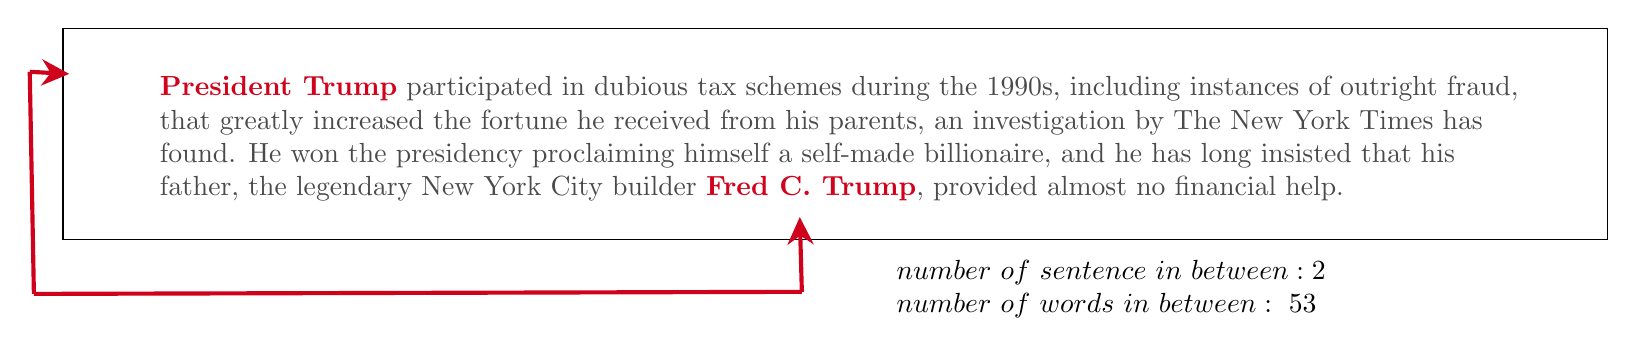
\begin{tikzpicture}[x=0.75pt,y=0.75pt,yscale=-1,xscale=1]
%uncomment if require: \path (0,300); %set diagram left start at 0, and has height of 300

%Shape: Rectangle [id:dp04377104671850285] 
\draw   (28,32) -- (772,32) -- (772,134) -- (28,134) -- cycle ;
%Straight Lines [id:da6182552655813487] 
\draw [color={rgb, 255:red, 208; green, 2; blue, 27 }  ,draw opacity=1 ][line width=1.5]    (28,53.84) -- (12,53) ;

\draw [shift={(31,54)}, rotate = 183.01] [fill={rgb, 255:red, 208; green, 2; blue, 27 }  ,fill opacity=1 ][line width=1.5]  [draw opacity=0] (13.4,-6.43) -- (0,0) -- (13.4,6.44) -- (8.9,0) -- cycle    ;
%Straight Lines [id:da6143692538402417] 
\draw [color={rgb, 255:red, 208; green, 2; blue, 27 }  ,draw opacity=1 ][line width=1.5]    (12,53) -- (14,160) ;


%Straight Lines [id:da10338493648199298] 
\draw [color={rgb, 255:red, 208; green, 2; blue, 27 }  ,draw opacity=1 ][line width=1.5]    (384,159) -- (14,160) ;


%Straight Lines [id:da054560662392693526] 
\draw [color={rgb, 255:red, 208; green, 2; blue, 27 }  ,draw opacity=1 ][line width=1.5]    (383.08,126) -- (384,159) ;

\draw [shift={(383,123)}, rotate = 88.41] [fill={rgb, 255:red, 208; green, 2; blue, 27 }  ,fill opacity=1 ][line width=1.5]  [draw opacity=0] (13.4,-6.43) -- (0,0) -- (13.4,6.44) -- (8.9,0) -- cycle    ;

% Text Node
\draw (402,108) node [scale=1,color={rgb, 255:red, 74; green, 74; blue, 74 }  ,opacity=1 ] [align=left] {\textcolor[rgb]{0.82,0.01,0.11}{\textbf{President Trump}} participated in dubious tax schemes during the 1990s, including instances of outright fraud, \\that greatly increased the fortune he received from his parents, an investigation by The New York Times has\\found. He won the presidency proclaiming himself a self-made billionaire, and he has long insisted that his \\father, the legendary New York City builder \textcolor[rgb]{0.82,0.01,0.11}{\textbf{Fred C. Trump}}, provided almost no financial help.\\\\\\};
% Text Node
\draw (533,158) node   {$ \begin{array}{l}
number\ of\ sentence\ in\ between:2\\
number\ of\ words\ in\ between:\ 53
\end{array}$};


\end{tikzpicture}

}
\caption{An example text to show the relation between two actor entities, \emph{``Donald Trump"} and \emph{``Fred C. Trump"}. If the word-based window size is applied then the relationships between the two entities is not captured, even though they are only one sentence apart. }
\label{fig:article_entities}
\end{figure}
\section{Word Embeddings on Raw Text}\label{sec:raw}
State-of-the-art word embedding models are trained on raw text (without entity annotation). The word2vec and GloVe models, explained in Chapter~\ref{chap:background}, Sections~\ref{subsec:word2vec} and~\ref{subsec:GloVe} respectively, are chosen as representative of classical word embeddings.From the word2vec model, the skip-gram architecture is chosen. We refer to the word2vec and GloVe model as $rW2V$ and  $rGLV$, where \emph{``r"} denotes raw text input.The text is cleaned only by common pre-processing steps. The corpus is tokenized into words and stop words and punctuations are removed. Non-alphabetic characters, like Chinese or Arabic vocabulary, are disregard and multiple white spaces are reduced to only one.  Any HTML tags or numeric values are also removed from the text, to produce a clean document, containing only terms relevant to the model. In addition, all the words are converted to their lower-case form to avoid multiple representations of a single term. Since no entities are annotated, all words are treated as terms. 
\section{Word Embeddings on Annotated Text}\label{sec:annotated}
In Chapter~\ref{chap:intro}, we defined named entities $N$ as a subset of all terms $N\subseteq T$ that fall into a pre-defined category. In other words, terms that have a specific type are considered as named entities. Hence, the simplest way to obtain their embeddings would be to run the well-established word embedding models on the annotated text. Our contribution to these models is not the modification of the underlying method, but the input. The input of the model is no longer the raw text, but a corpus with annotated named entities. The task of annotation involves POS tagging, named entity recognition and disambiguation. Since word embeddings learn the representation for each token in the text, our definition of the token is changed. A token is no longer a single word separated by space but named entity with a specific type. Any word that does not fit into any of the pre-defined types is considered as a term. In the set $T$ multiple entities might share ambiguous labels, but after annotation they can be represented with a unique identifier. In our case, the identifier is the type of the word and numeric key, e.g,  \emph{ACT\_17}, for an actor. As a result, compound words, such as names of people and organizations are considered as one word. All mentions of  \emph{A\_17}, which corresponds to the actor  \emph{``Barack Obama"} are represented with a single notation. Thus, making the text less ambiguous. In addition, depending on the performance of the named entity recognition tool all other indirect mentions, e.g. \emph{``Mr. President"}, \emph{``President of the United States"}, are also replaced with their corresponding entity identifier. The same applies to different mentions of dates that result into date embeddings. Words that belong to more than one entity type, have an embedding for each type. For example, \emph{``Washington"} can either be a name of a person or a city and will have two separate embeddings for the actor and location context. The same strategy applies for terms, e.g,  \emph{TER\_22}.  Adding the type information in the name helps us identify and group named entities easier. \\
\begin{figure}
\centering 
\resizebox{0.85\textwidth}{0.28\textwidth}{      
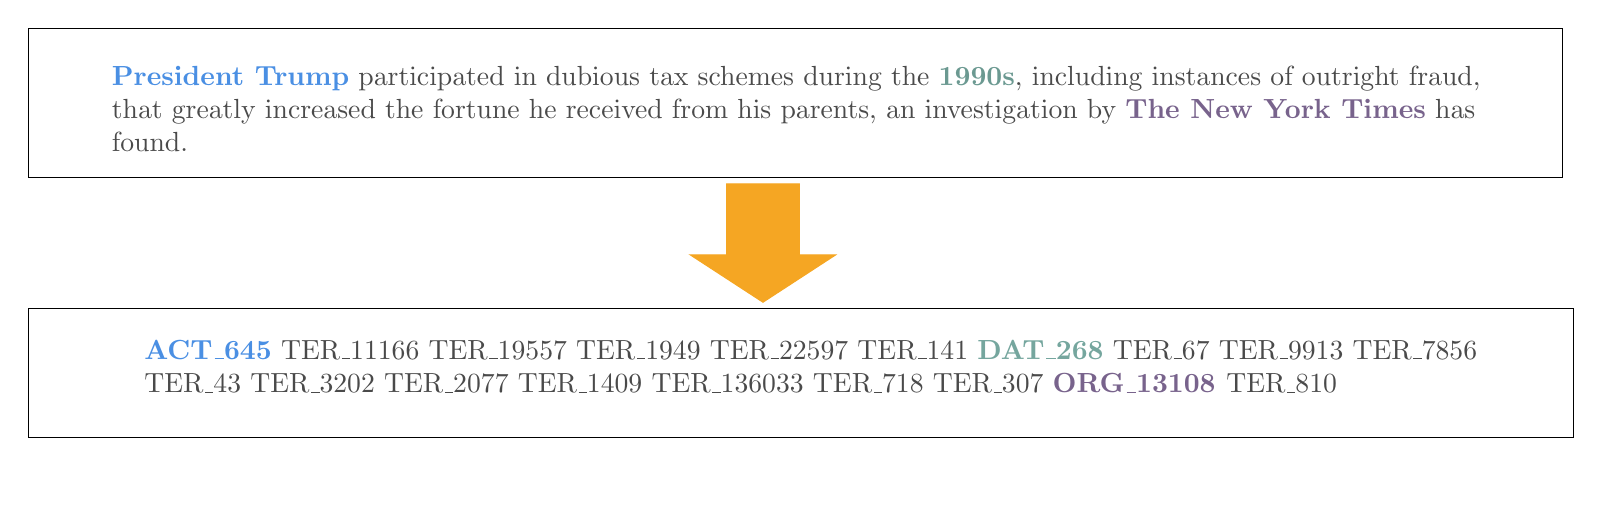
\begin{tikzpicture}[x=0.75pt,y=0.75pt,yscale=-1,xscale=1]
%uncomment if require: \path (0,377); %set diagram left start at 0, and has height of 377

%Shape: Rectangle [id:dp8906489990544584] 
\draw   (28,17) -- (767,17) -- (767,89) -- (28,89) -- cycle ;
%Shape: Rectangle [id:dp9074920271044917] 
\draw   (28,152) -- (772.5,152) -- (772.5,214) -- (28,214) -- cycle ;
%Down Arrow [id:dp1838486332286331] 
\draw  [color={rgb, 255:red, 245; green, 166; blue, 35 }  ,draw opacity=1 ][fill={rgb, 255:red, 245; green, 166; blue, 35 }  ,fill opacity=1 ] (347,126.2) -- (364.5,126.2) -- (364.5,92) -- (399.5,92) -- (399.5,126.2) -- (417,126.2) -- (382,149) -- cycle ;

% Text Node
\draw (398,80) node [scale=1,color={rgb, 255:red, 74; green, 74; blue, 74 }  ,opacity=1 ] [align=left] {\textcolor[rgb]{0.29,0.56,0.89}{\textbf{President Trump}} participated in dubious tax schemes during the \textcolor[rgb]{0.42,0.6,0.57}{\textbf{1990s}}, including instances of outright fraud, \\that greatly increased the fortune he received from his parents, an investigation by \textcolor[rgb]{0.47,0.39,0.55}{\textbf{The New York Times}} has\\found. \\\\\\};
% Text Node
\draw (405,204) node [scale=1,color={rgb, 255:red, 74; green, 74; blue, 74 }  ,opacity=1 ] [align=left] {\textbf{\textcolor[rgb]{0.29,0.56,0.89}{ACT\_645}} TER\_11166 TER\_19557 TER\_1949 TER\_22597 TER\_141 \textbf{\textcolor[rgb]{0.46,0.65,0.62}{DAT\_268}} TER\_67 TER\_9913 TER\_7856 \\TER\_43 TER\_3202 TER\_2077 TER\_1409 TER\_136033 TER\_718 TER\_307 \textbf{\textcolor[rgb]{0.47,0.39,0.55}{ORG\_13108} }TER\_810\\\\\\};


\end{tikzpicture}

}
\caption{An example of the pre-processing for annotated text. All the entity mentions are replaced with their unique identifier and the unnecessary tags POS-tags are removed. }
\label{fig:annotation}
\end{figure}
Since entity annotation requires POS tagging, we used the POS tags to remove stop-word, punctuation. After annotation all the entities are replaced with their unique identifier and remaining words are considered as terms ($T\setminus  N$). An example of the text after annotation and pre-processing is shown in Figure~\ref{fig:annotation}. After annotation, we use word2vec and GloVe and refer to them as $aW2V$ and $aGLV$, where \emph{``a"} denotes the use of annotated text. 
%
%For text pre-processing, punctuation and stop-word are removed and terms in the text are filtered to a certain POS-tag. Unnecessary tags are removed, namely  wh-determiner, wh-pronouns, wh-adverbs, common verbs, such as  \emph{have} and  \emph{do} in past or present, interjections (e.g. ah!, dear me!) and other terms that mostly fall into stop-words category such as: predeterminer (both and a lot of), possessive endings and prepositions (until, before,...), determiner (a, the, every) and coordinating conjunction (and, but, or). 

\section{Node Embeddings of Cooccurrence Graphs}\label{sec:graph_based}
We defined a co-occurrence graph of words in Chapter~\ref{chap:background}, as a graph $G=(T,E)$, where $T$ is the set of terms in the vocabulary as nodes and $E$ set of edges and the edge weights encode some notion of distance between the words. We extract such graph from the textual corpus with named-entity annotations. As a result, we obtain a weighted heterogeneous graph $G=(N,E)$ of named entity, where the set $N$ contains entities of different types and terms. For entity annotations in particular, implicit networks can serve as graph representations. By using stenece-window for finding the relationship between entities, they can capture entity relations even stentences apart. ~\brackettext{\cite{DBLP:conf/sigir/SpitzG16}}. Thus, by embedding the nodes, we can obtain word embeddings for both terms and entities.  We later show that this method achieves a better performance in comparison to $W2Vr$ and $GLVr$ on the annotated text. For the node embeddings, we chose DeepWalk ($DW$) and VERSE ($VRS$), explained in Chapter~\ref{chap:background}, Sections~\ref{subsec:DeepWalk} and ~\ref{subsec:VERSE} respectively. However, since we work on weighted graphs and weights display the strength of the relationships, weighted random walks are introduced to replace the uniform random walk in the DeepWalk model. The probability of a node visiting its neighbors is proportional to the edge weight. As a result, the probability of visiting node $j$ from vertex $i$ with edge weight $e_{i,j}$,  is given in Equation~\ref{eq:edge_weight}, where $ E_{ i }$ denotes the set of all edges starting from node $t_{i}$. The stronger the relationship, the more probable is it to be visited. 
\begin{equation}
P_{i,j}=\frac{e_{i,j}}{\sum _{ e_{ k }\in E_{ i } }^{  }{ e_{k} } }
\label{eq:edge_weight}
\end{equation}
In a word co-occurrence
graph, some words co-occur many times and some only a few times. Therefore, the weights can fluctuate between small numbers up to tens of thousands, resulting in highly unbalanced transition probabilities, causing some nodes to never be visited in a random walk. To solve this issue and create a more balanced weight distribution, $ \log$ mapping is used. In the $\log$ mapping, all edge weights are replaced by their logarithm and the transition probabilities are computed accordingly. We refer to the DeepWalk with $log$ mapping as ($DW_{log}$) and without $log$ mapping as ($DW_{id}$). Because of the unbalanced weight distribution, the optimization objective for the second-order proximity of LINE model becomes ill-defined. Hence, one part of the embedding for this model cannot be trained properly and since only half an embedding does not represent the model we did not use it for generating entity embeddings. \\
\begin{figure}
\centering 
\resizebox{0.50\textwidth}{0.35\textwidth}{      
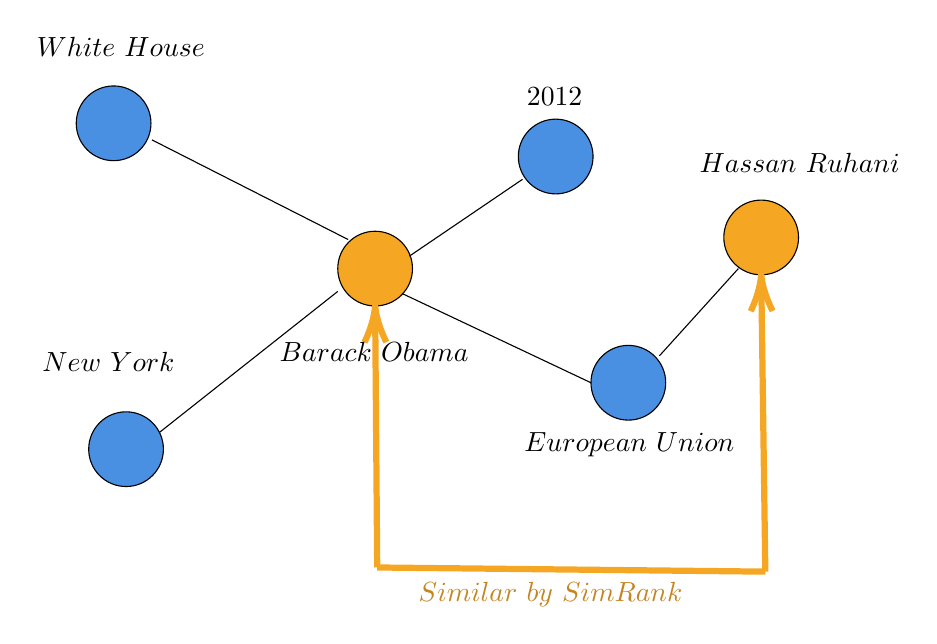
\begin{tikzpicture}[x=0.75pt,y=0.75pt,yscale=-1,xscale=1]
%uncomment if require: \path (0,407); %set diagram left start at 0, and has height of 407

%Shape: Circle [id:dp7237033228697587] 
\draw  [color={rgb, 255:red, 0; green, 0; blue, 0 }  ,draw opacity=1 ][fill={rgb, 255:red, 74; green, 144; blue, 226 }  ,fill opacity=1 ] (142.5,97) .. controls (142.5,87.06) and (150.56,79) .. (160.5,79) .. controls (170.44,79) and (178.5,87.06) .. (178.5,97) .. controls (178.5,106.94) and (170.44,115) .. (160.5,115) .. controls (150.56,115) and (142.5,106.94) .. (142.5,97) -- cycle ;
%Straight Lines [id:da7651994649420626] 
\draw    (179,105) -- (273.5,153) ;


%Shape: Circle [id:dp1628508691866306] 
\draw  [color={rgb, 255:red, 0; green, 0; blue, 0 }  ,draw opacity=1 ][fill={rgb, 255:red, 74; green, 144; blue, 226 }  ,fill opacity=1 ] (148.5,254) .. controls (148.5,244.06) and (156.56,236) .. (166.5,236) .. controls (176.44,236) and (184.5,244.06) .. (184.5,254) .. controls (184.5,263.94) and (176.44,272) .. (166.5,272) .. controls (156.56,272) and (148.5,263.94) .. (148.5,254) -- cycle ;
%Shape: Circle [id:dp6369036191517297] 
\draw  [color={rgb, 255:red, 0; green, 0; blue, 0 }  ,draw opacity=1 ][fill={rgb, 255:red, 245; green, 166; blue, 35 }  ,fill opacity=1 ] (268.5,167) .. controls (268.5,157.06) and (276.56,149) .. (286.5,149) .. controls (296.44,149) and (304.5,157.06) .. (304.5,167) .. controls (304.5,176.94) and (296.44,185) .. (286.5,185) .. controls (276.56,185) and (268.5,176.94) .. (268.5,167) -- cycle ;
%Shape: Circle [id:dp6138711151460285] 
\draw  [color={rgb, 255:red, 0; green, 0; blue, 0 }  ,draw opacity=1 ][fill={rgb, 255:red, 74; green, 144; blue, 226 }  ,fill opacity=1 ] (390.5,222) .. controls (390.5,212.06) and (398.56,204) .. (408.5,204) .. controls (418.44,204) and (426.5,212.06) .. (426.5,222) .. controls (426.5,231.94) and (418.44,240) .. (408.5,240) .. controls (398.56,240) and (390.5,231.94) .. (390.5,222) -- cycle ;
%Shape: Circle [id:dp15908024717263558] 
\draw  [color={rgb, 255:red, 0; green, 0; blue, 0 }  ,draw opacity=1 ][fill={rgb, 255:red, 74; green, 144; blue, 226 }  ,fill opacity=1 ] (355.5,113) .. controls (355.5,103.06) and (363.56,95) .. (373.5,95) .. controls (383.44,95) and (391.5,103.06) .. (391.5,113) .. controls (391.5,122.94) and (383.44,131) .. (373.5,131) .. controls (363.56,131) and (355.5,122.94) .. (355.5,113) -- cycle ;
%Straight Lines [id:da4548959711882159] 
\draw    (303,161) -- (357.5,124) ;


%Straight Lines [id:da6860631222603604] 
\draw    (299.5,179) -- (390.5,222) ;


%Straight Lines [id:da5778462671903315] 
\draw    (423.5,209) -- (461.5,167) ;


%Shape: Circle [id:dp9805133554604324] 
\draw  [color={rgb, 255:red, 0; green, 0; blue, 0 }  ,draw opacity=1 ][fill={rgb, 255:red, 245; green, 166; blue, 35 }  ,fill opacity=1 ] (454.5,152) .. controls (454.5,142.06) and (462.56,134) .. (472.5,134) .. controls (482.44,134) and (490.5,142.06) .. (490.5,152) .. controls (490.5,161.94) and (482.44,170) .. (472.5,170) .. controls (462.56,170) and (454.5,161.94) .. (454.5,152) -- cycle ;
%Straight Lines [id:da3078528737086299] 
\draw    (182.5,246) -- (268.5,178) ;


%Straight Lines [id:da6689641936732076] 
\draw [color={rgb, 255:red, 245; green, 166; blue, 35 }  ,draw opacity=1 ][line width=2.25]    (287.5,311) -- (286.53,189) ;
\draw [shift={(286.5,185)}, rotate = 449.55] [color={rgb, 255:red, 245; green, 166; blue, 35 }  ,draw opacity=1 ][line width=2.25]    (17.49,-5.26) .. controls (11.12,-2.23) and (5.29,-0.48) .. (0,0) .. controls (5.29,0.48) and (11.12,2.23) .. (17.49,5.26)   ;

%Straight Lines [id:da23704536821016675] 
\draw [color={rgb, 255:red, 245; green, 166; blue, 35 }  ,draw opacity=1 ][line width=2.25]    (474.5,313) -- (472.56,174) ;
\draw [shift={(472.5,170)}, rotate = 449.2] [color={rgb, 255:red, 245; green, 166; blue, 35 }  ,draw opacity=1 ][line width=2.25]    (17.49,-5.26) .. controls (11.12,-2.23) and (5.29,-0.48) .. (0,0) .. controls (5.29,0.48) and (11.12,2.23) .. (17.49,5.26)   ;

%Straight Lines [id:da7509045062366104] 
\draw [color={rgb, 255:red, 245; green, 166; blue, 35 }  ,draw opacity=1 ][line width=2.25]    (287.5,311) -- (474.5,313) ;



% Text Node
\draw (164,60) node   {$White\ House$};
% Text Node
\draw (286,207) node   {$Barack\ Obama$};
% Text Node
\draw (409,252) node   {$European\ Union$};
% Text Node
\draw (491,116) node   {$Hassan\ Ruhani$};
% Text Node
\draw (158,212) node   {$New\ York$};
% Text Node
\draw (373,84) node   {$2012$};
% Text Node
\draw (371,324) node [color={rgb, 255:red, 196; green, 133; blue, 33 }  ,opacity=1 ]  {$Similar\ by\ SimRank$};


\end{tikzpicture}


}
\caption{An example of SimRank similarity. In this graph, although the relationship between the president of Iran and the US is discovered by SimRank, the more important relationships, namely direct neighbors are disregarded. The similarity between \emph{``Barack Obama"} and the direct neighbors are zero.  }
\label{fig:simrank}
\end{figure}
The VERSE model does not support the incorporation of the edge weights. From the three similarity measure that VERSE offers, we chose Adjacency Similarity to produce the entity embeddings. Our reason is two-folded: first, the PPR relates to the stationary distribution of a random walk with restart and we already represented the random walk-based models with DeepWalk. Second, SimRank is a measure of structural relatedness, between two nodes, based on the assumption that two nodes are
similar if they are connected to other similar nodes. Although words that happen often with the same words can themselves be considered similar, if we only look at nodes that have common neighbors we lose most of the adjacency relations in the graph. An example is illustrated in Figure~\ref{fig:simrank}. Since the SimRank of two nodes with no common neighbor, is zero, the direct neighbors are disregarded. However, SimRank tends to discover interesting relationship, such as the one shown in Figure~\ref{fig:simrank} and possibly if a new similarity measure is introduced that creates a trade-off between SimRank and Adjacency Similarity, the results might improve. For this study, however, we choose only Adjacency Similarity to learn the embeddings. Adjacency Similarity is based on the normalized adjacency matrix and captures the neighborhood relations. Moreover, it correlates with the first-order proximity in LINE and can be used as representative of first-order proximity. \\
\section{Similarity Between Embeddings }\label{sec:similarity}
The dense word vector is learned to capture the semantics of the words and hence similar words are close in the induced space. \emph{cosine similarity} helps to capture this semantic closeness and is the most common similarity measure for the word vector. The cosine similarity is a measure that calculates the cosine of the angle between two vectors. This metric is a measurement of orientation and not magnitude and it is derived from the equation of a dot product between two vectors (Equation~\ref{eq:cosine}). The vectors are normalized by their length, which removes the influence of their magnitude on the similarity. The norm of the vector is somewhat related to the overall frequency of which words occur in the training corpus, but the direction is unaffected by this. So in order for a common word like \emph{``frog"} to still be similar to a less frequent word like \emph{``Anura"} (a type of frog), cosine distance which only looks at the direction works better than simple Euclidean distance. Moreover, cosine similarity is symmetric and changing the order of vectors in the dot product does not effect the final result.
\begin{equation}
\begin{split}
\overrightarrow { w_a } .\overrightarrow { w_b } =\parallel \overrightarrow { w_a } \parallel \parallel \overrightarrow { w_b } \parallel cos\theta 
\\
cos\theta =\frac { \overrightarrow { w_a } .\overrightarrow { w_b }  }{ \parallel \overrightarrow { w_a } \parallel \parallel \overrightarrow { w_b } \parallel  } 
\end{split}
\label{eq:cosine}
\end{equation}
\noindent
In this chapter,  two methods to extract entity and term embeddings from an annotated corpus were introduced. One method learns the embeddings directly from the text, while the other one generates a co-occurrence graph and embeds the nodes. In the next Chapter we attempt to create embeddings separable by entity type and in In Chapter~\ref{chap:eval}, we report the evaluation results for both entity and facetted embeddings. We also show why the extraction of a co-occurrence graph is crucial for achieving better performance. 